% vim: set spell spelllang=es syntax=tex :

\documentclass[11pt,a4paper,spanish]{beamer}

\usepackage[spanish]{babel}

\usepackage[utf8]{inputenc}

\usepackage{graphicx}

\usepackage{subcaption} %Para Subfigure

\usepackage{caption} %Para captions en las figuras sin prefijo

\usepackage{ccicons}

\usepackage{url}

\usepackage{babelbib}

\usefonttheme{serif}

\setlength{\parskip}{1.5mm}

\newcommand{\codeword}[1]{\mbox{\texttt{\textcolor{blue}{#1}}}}
\newcommand{\dq}[0]{\textquotesingle\hspace{-0.25em}\textquotesingle}
\newcommand{\sq}[0]{\textquotesingle}

\usetheme{Rochester}
\usecolortheme{whale}

%\usetheme{Warsaw}

\beamertemplatenavigationsymbolsempty

\setbeamertemplate{background canvas}{
    \raisebox{-0.99\paperheight}[0pt][0pt]{
        \makebox[\paperwidth]{
            \null
            \hspace{-1em}
            
\includegraphics[width=0.09\paperwidth]{logos/fai.pdf}
            \hspace{0.8\paperwidth}
            %\hfill
            \hspace{-1em}
            \includegraphics[width=0.09\paperwidth]{logos/uncoma.pdf}
            }
    }
}

\title{\textbf{Administración de cuentas de usuarios}}

\author{}

\date{}

\defbeamertemplate{footline}{centered page number}
{
    \hspace*{\fill}
    \usebeamercolor[fg]{blue}
    \usebeamerfont{page number in head/foot}
    \insertpagenumber\,/\,\insertpresentationendpage
    \hspace*{\fill}\vskip2pt
}
\setbeamertemplate{footline}[centered page number]

\begin{document}

\begin{frame}[noframenumbering]

    \maketitle
    %\centering
    %\vspace{-8em}~
    %\begin{figure}
    %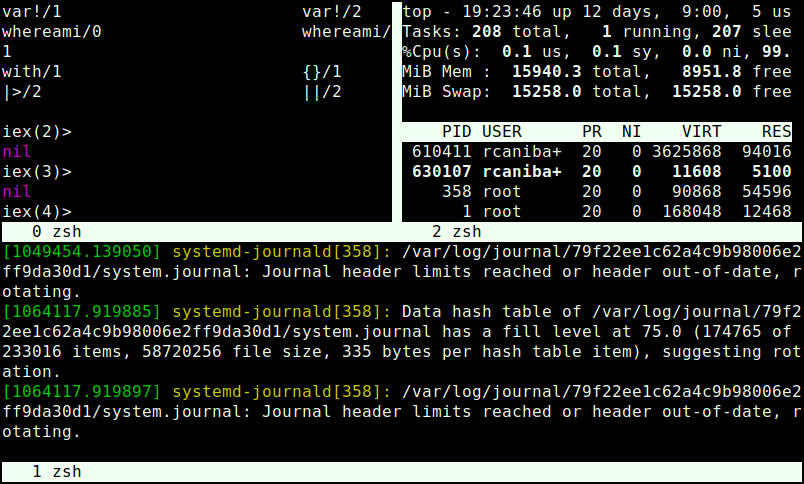
\includegraphics[height=0.55\textheight]{img/screen.pdf}
    %\end{figure}

\end{frame}

\begin{frame}[label=temario]

    \frametitle{Temario}

\begin{itemize}

    \item Definición de cuenta de usuario.
    \item Archivos de configuración.
    \item Proceso de alta, baja, y modificación de un usuario.
        \begin{itemize}
            \item Proceso manual.
            \item Herramientas del sistema.
        \end{itemize}

\end{itemize}

\end{frame}

\begin{frame}

    \frametitle{Definición de cuenta de usuario}

    Una \emph{cuenta de usuario} esta compuesta por:
    \begin{itemize}
        \item Nombre de usuario: una cadena de texto alfanumérica única.
        \item Contraseña.
        \item Archivos de usuario y de configuración.
    \end{itemize}

    Internamente el sistema utiliza un número de identificador único para
    identificar al usuario (\emph{uid}).

\end{frame}

\begin{frame}

    \frametitle{Archivos de configuración}

    \begin{itemize}
        \item \codeword{/etc/passwd}: Contiene la lista de usuarios del sistema y la
            información básica de estos (ver \codeword{man 5 passwd}).
        \item \codeword{/etc/shadow}: Información de las contraseñas de los
            usuarios (ver \codeword{man 5 shadow}).
        \item \codeword{/etc/group}: Contiene la lista de los grupos de
            sistema e información de la pertenencia de los usuarios a estos
            (ver \codeword{man 5 group}).
        \item \codeword{/etc/skel}: Directorio que contiene los archivos
            predefinidos para un nuevo usuario.
    \end{itemize}

\end{frame}

\begin{frame}

    \frametitle{Archivos de configuración}
    \framesubtitle{/etc/passwd}

    Es archivo de texto, legible por todos los usuarios, donde cada linea
    corresponde a un usuario, y que contiene los siguientes campos separados
    por el caracter dos puntos (``\codeword{:}''):

    \begin{enumerate}
        \setcounter{enumi}{-1}
        \item Nombre de usuario.
        \item Opcionalmente, el hash de la contraseña.
        \item Número de identificación del usuario.
        \item Número de identificación del grupo primario.
        \item Nombre completo.
        \item Directorio \codeword{HOME}.
        \item \codeword{shell} de login del usuario.
    \end{enumerate}

\end{frame}

\begin{frame}

    \frametitle{Archivos de configuración}
    \framesubtitle{/etc/shadow}

    Es archivo de texto, solo legible por \codeword{root}, donde cada linea
    corresponde a un usuario, y que contiene los siguientes campos separados
    por el caracter dos puntos (``\codeword{:}''):

    \begin{enumerate}
        \setcounter{enumi}{-1}
        \item Nombre de usuario.
        \item El hash de la contraseña.
        \item Fecha del último cambio de contraseña.
        \item Tiempo mínimo antes permitir cambio de contraseña.
        \item Tiempo máximo antes de pedir cambio de contraseña.
        \item Periodo de notificación previo del vencimiento de la contraseña.
        \item Periodo de gracia luego del vencimiento de la contraseña.
        \item Fecha de expiración de la cuenta.
        \item Campo reservado para usos futuros.
    \end{enumerate}

\end{frame}

\begin{frame}

    \frametitle{Archivos de configuración}
    \framesubtitle{/etc/group}

    Es archivo de texto, legible por todos los usuarios, donde cada linea
    corresponde a un grupo, y que contiene los siguientes campos separados por
    el caracter dos puntos (``\codeword{:}''):

    \begin{enumerate}
        \setcounter{enumi}{-1}
        \item Nombre del grupo.
        \item Opcionalmente, el hash de la contraseña del grupo.
        \item Número de identificación del grupo.
        \item Lista de los usuarios que pertenecen al grupo, separados por
            coma.
    \end{enumerate}

\end{frame}

\begin{frame}

    \frametitle{Alta, baja, y modificación de usuarios}
    \framesubtitle{Creación manual}

    \begin{enumerate}
        \item Crear una nueva linea en el archivo \codeword{/etc/passwd}.
            Colocar una \codeword{x} en el campo de contraseña. Verificar que
            el usuario y \emph{uid} son únicos. Editar con \codeword{vipw}.
        \item Crear una nueva linea en el archivo \codeword{/etc/shadow}.
            Colocar una \codeword{!} en el campo de contraseña. Editar con
            \codeword{vipw -s}.
        \item Agregar el usuario a su grupo primario y secundarios en
            \codeword{/etc/group}. Editar con \codeword{vigr}.
        \item Utilizar el comando \emph{passwd -e \$NewUser} para asignarle
            una contraseña valida al usuario.
        \item Crear el directorio \codeword{HOME} del usuario y copiar los
            contenidos del directorio \codeword{/etc/skel} a este.
        \item Asignar al nuevo usuario como dueño del su directorio
            \codeword{HOME}.
    \end{enumerate}

\end{frame}

\begin{frame}

    \frametitle{Alta, baja, y modificación de usuarios}
    \framesubtitle{Deshabilitación manual}

    \begin{itemize}
        \item Agregar un caracter \codeword{!} o \codeword{*} delante de la
            contraseña en el archivo \codeword{/etc/shadow}. El usuario no
            podrá ingresar al sistema por medio de su contraseña
            \codeword{UNIX}, pero si por otros medios.
        \item Cambiar el \codeword{shell} del usuario por
            \codeword{/sbin/nologin} o \codeword{/bin/false}. El usuario se
            identificara satisfactoriamente, pero no podrá ingresar por medio
            de las terminales virtuales.
    \end{itemize}

\end{frame}

\begin{frame}

    \frametitle{Alta, baja, y modificación de usuarios}
    \framesubtitle{Herramientas del sistema}

    \begin{itemize}
        \item \codeword{useradd} y \codeword{adduser}: Crean un nuevo usuario.
            \codeword{adduser} crea el directorio \codeword{HOME} y copia los
            archivos de \codeword{/etc/skel}.
        \item \codeword{chsh}: Cambia el \codeword{shell} del
            usuario\footnote{un usuario puede usar este comando para modificar
            sus propios atributos\label{fnCHSH}}.
        \item \codeword{passwd}: Cambia la contraseña del
            usuario\textsuperscript{\ref{fnCHSH}}.
        \item \codeword{usermod}: Modifica cualquier campo del usuario.
        \item \codeword{userdel} y \codeword{deluser}: Borran un usuario.
            \codeword{deluser} tiene opciones para borrar todos los archivos
            del usuario.
    \end{itemize}

\end{frame}

\againframe{temario}

\begin{frame}

\title{¿Consultas?}
\maketitle

\end{frame}
%
%\newcounter{lastPage}
%\setcounter{lastPage}{\number\value{page}}
%
%\begin{frame}%[allowframebreaks]
%
%\frametitle{Atribuciones}
%
%\bibliographystyle{abbrv}
%\setbeamertemplate{bibliography item}{\insertbiblabel}
%\tiny
%\bibliography{refimg}
%\end{frame}
%
%\setcounter{page}{\number\value{lastPage}}

\end{document}
